
%-----------------------------------------------------------------------
\section{Transforming}
%-----------------------------------------------------------------------
%
% UML Transformation overview
%
\frame
{
  \frametitle{Transformation overview}

\begin{center}
\begin{figure}
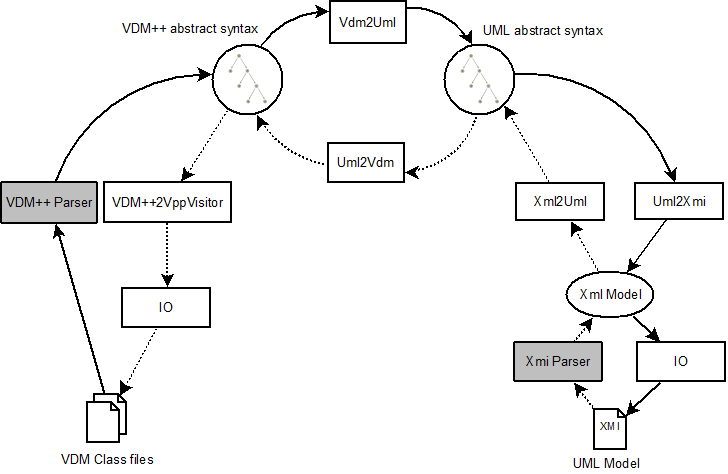
\includegraphics[width=\textwidth]{images/OverviewOverMapping.png}
\end{figure}
\end{center}
}
%-----------------------------------------------------------------------
\subsection{Transforming VDM++ to UML}
%-----------------------------------------------------------------------

%
% Transformation
%
\frame
{
  \frametitle{Transformation from VDM to UML}

\begin{center}
	\begin{block}<+->{Not created yet}
	Some thing about VDM
	\end{block}

\end{center}
}


%
% UML Transformation overview to VDM
%
\frame
{
  \frametitle{Transformation overview}
\begin{center}
\begin{figure}

\includegraphics<1->[width=\textwidth]{images/OverviewOverMapping.png}%
\llap{\includegraphics<2->[width=\textwidth]{images/OverviewOverMappingToVDM1.png}}%
\llap{\includegraphics<3->[width=\textwidth]{images/OverviewOverMappingToVDM2.png}}%
\llap{\includegraphics<4->[width=\textwidth]{images/OverviewOverMappingToVDM3.png}}%
\llap{\includegraphics<5->[width=\textwidth]{images/OverviewOverMappingToVDM4.png}}%

\end{figure}
\end{center}
}



%-----------------------------------------------------------------------
\subsection{Transforming UML to VDM++}
%-----------------------------------------------------------------------
%
% Transformation
%
\frame
{
  \frametitle{Transformation from UML to VDM}

\begin{center}
	\begin{block}<+->{Not created yet}
	Some thing about VDM
	\end{block}

\end{center}
}



%
% UML Transformation overview to UML
%
\frame
{
  \frametitle{Transformation overview}
\begin{center}
\begin{figure}

\includegraphics<1->[width=\textwidth]{images/OverviewOverMapping.png}%
\llap{\includegraphics<2->[width=\textwidth]{images/OverviewOverMappingToUML1.png}}%
\llap{\includegraphics<3->[width=\textwidth]{images/OverviewOverMappingToUML2.png}}%
\llap{\includegraphics<4->[width=\textwidth]{images/OverviewOverMappingToUML3.png}}%
\llap{\includegraphics<5->[width=\textwidth]{images/OverviewOverMappingToUML4.png}}%
\llap{\includegraphics<6->[width=\textwidth]{images/OverviewOverMappingToUML5.png}}%

\end{figure}
\end{center}
}

%-----------------------------------------------------------------------
\subsection{Merging}
%-----------------------------------------------------------------------
%
% Merging
%
\frame
{
  \frametitle{Merging}

\begin{center}
	\begin{block}<+->{Merging models}
	Do we want to spend a slide on this.
	\end{block}

\begin{figure}
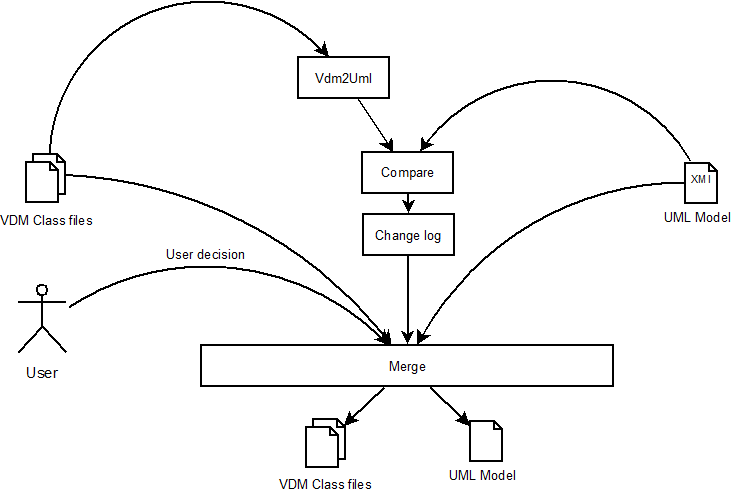
\includegraphics[width=0.6\textwidth]{images/Merge.png}
\end{figure}

\end{center}
}



